%%%%%%%%%%%%%%%%%%%%%%%%%%%%%%%%%%%%%%%%%
% Jacobs Landscape Poster
% LaTeX Template
% Version 1.1 (14/06/14)
%
% Created by:
% Computational Physics and Biophysics Group, Jacobs University
% https://teamwork.jacobs-university.de:8443/confluence/display/CoPandBiG/LaTeX+Poster
%
% Further modified by:
% Nathaniel Johnston (nathaniel@njohnston.ca)
%
% This template has been downloaded from:
% http://www.LaTeXTemplates.com
%
% License:
% CC BY-NC-SA 3.0 (http://creativecommons.org/licenses/by-nc-sa/3.0/)
%
%%%%%%%%%%%%%%%%%%%%%%%%%%%%%%%%%%%%%%%%%

%----------------------------------------------------------------------------------------
%	PACKAGES AND OTHER DOCUMENT CONFIGURATIONS
%----------------------------------------------------------------------------------------

\documentclass[xcolor=table,final]{beamer}

\usepackage[scale=1.15]{beamerposter} % Use the beamerposter package for laying out the poster


\usetheme{confposter} % Use the confposter theme supplied with this template

\setbeamercolor{block title}{fg=jblue,bg=white} % Colors of the block titles
\setbeamercolor{block body}{fg=black,bg=white} % Colors of the body of blocks
\setbeamercolor{block alerted title}{fg=white,bg=dblue!70} % Colors of the highlighted block titles
\setbeamercolor{block alerted body}{fg=black,bg=dblue!10} % Colors of the body of highlighted blocks
% Many more colors are available for use in beamerthemeconfposter.sty

%-----------------------------------------------------------
% Define the column widths and overall poster size
% To set effective sepwid, onecolwid and twocolwid values, first choose how many columns you want and how much separation you want between columns
% In this template, the separation width chosen is 0.024 of the paper width and a 4-column layout
% onecolwid should therefore be (1-(# of columns+1)*sepwid)/# of columns e.g. (1-(4+1)*0.024)/4 = 0.22
% Set twocolwid to be (2*onecolwid)+sepwid = 0.464
% Set threecolwid to be (3*onecolwid)+2*sepwid = 0.708

\newlength{\sepwid}
\newlength{\onecolwid}
\newlength{\twocolwid}
\newlength{\threecolwid}
\setlength{\paperwidth}{46.8in} % A0 width: 46.8in
\setlength{\textwidth}{44.8in}
\setlength{\paperheight}{33.1in} % A0 height: 33.1in
\setlength{\textwidth}{31.1in}
\setlength{\sepwid}{0.024\paperwidth} % Separation width (white space) between columns
\setlength{\onecolwid}{0.22\paperwidth} % Width of one column
\setlength{\twocolwid}{0.464\paperwidth} % Width of two columns
\setlength{\threecolwid}{0.708\paperwidth} % Width of three columns
\setlength{\topmargin}{-0.5in} % Reduce the top margin size

%-----------------------------------------------------------


\usepackage{booktabs} % Top and bottom rules for tables

\makeatletter
\let\@@magyar@captionfix\relax
\makeatother

\usepackage[backend=bibtex,style=numeric,maxnames=3]{biblatex}
\addbibresource{main.bib}

\usepackage{graphicx}
\usepackage{subfig}

% Matrix decomposition diagram
\usepackage{stackengine}
\stackMath
\newlength\matfield
\newlength\tmplength
\def\matscale{1.}
\newcommand\dimbox[3]{%
  \setlength\matfield{\matscale\baselineskip}%
  \setbox0=\hbox{\vphantom{X}\smash{#3}}%
  \setlength{\tmplength}{#1\matfield-\ht0-\dp0}%
  \fboxrule=1pt\fboxsep=-\fboxrule\relax%
  \fbox{\makebox[#2\matfield]{\addstackgap[.5\tmplength]{\box0}}}%
}
\newcommand\raiserows[2]{%
   \setlength\matfield{\matscale\baselineskip}%
   \raisebox{#1\matfield}{#2}%
}
\newcommand\matbox[5]{
  \stackunder{\dimbox{#1}{#2}{$#5$}}{\scriptstyle(#3\times #4)}%
}
\parskip 1em

\usepackage{siunitx} % For scientific notation of p-values using \num

\usepackage{tabularx}
% Tables with merged vertical cells
\usepackage{multirow}

\setbeamerfont{block title}{size=\LARGE}
\setbeamerfont{caption}{size=\footnotesize}
\AtBeginBibliography{\footnotesize}
\setbeamertemplate{caption}[numbered]

% set colors for alerted blocks (blocks with frame)
\setbeamercolor{block alerted title}{fg=white,bg=nred}
\setbeamercolor{block alerted body}{fg=black,bg=nred!10}

\renewcommand{\bold}[1]{{\textcolor{norange}{\textbf{#1}}}}
\newcommand{\runnerup}[1] {\underline{\textit{#1}}}
\newcommand{\bestscore}[1] {\underline{\textbf{#1}}}

\setbeamercolor{subheading}{use=structure,fg=white,bg=norange}
\newcommand{\kcnsubheading}[1]{\begin{beamercolorbox}[rounded=true]{subheading}{\large #1}\end{beamercolorbox}}

%----------------------------------------------------------------------------------------
%	TITLE SECTION
%----------------------------------------------------------------------------------------

\newcommand{\samelineand}{\qquad}

\title{Comparison of sparse biclustering algorithms for gene expression datasets} % Poster title
\author{Katherine Nicholls \inst{1} \inst{2} and Chris Wallace \inst{1} \inst{2}}

\institute[shortinst]{\inst{1} Cambridge Institute for Therapeutic Immunology and Infectious Disease, University of Cambridge, Cambridge, CB2 0AW, UK \inst{2} MRC Biostatistics Unit, Cambridge Biomedical Campus, Forvie Site, Robinson Way, Cambridge, CB2 0SR, UK}

%----------------------------------------------------------------------------------------

\begin{document}

\addtobeamertemplate{block end}{}{\vspace*{2ex}} % White space under blocks
\addtobeamertemplate{block alerted end}{}{\vspace*{2ex}} % White space under highlighted (alert) blocks

%\setlength{\belowcaptionskip}{2ex} % White space under figures
\setlength\belowdisplayshortskip{2ex} % White space under equations


\begin{frame}[t] % The whole poster is enclosed in one beamer frame

\begin{columns}[t] % The whole poster consists of three major columns, the second of which is split into two columns twice - the [t] option aligns each column's content to the top

\begin{column}{\sepwid}\end{column} % Empty spacer column

\begin{column}{\onecolwid} % The first column

%----------------------------------------------------------------------------------------
%	INTRODUCTION
%----------------------------------------------------------------------------------------

\begin{block}{Why biclustering?}

Biclusters: groups of \bold{genes that covary} in a \bold{subset of the samples}.

\begin{itemize}
    \item Detects patterns not visible with gene clustering
    \item Provides link between samples and gene groups
    \item Adjusts for confounders
\end{itemize}

\begin{figure}
    \captionsetup[subfigure]{justification=centering}
\begin{minipage}{1\linewidth}
    \centering
\subfloat[Original matrix \label{fig:raw}]{
    
\includegraphics[width=0.2\textwidth]{plots/biclustering_diagrams/raw.png}}
\subfloat[Clustering genes\label{fig:rows}]{
    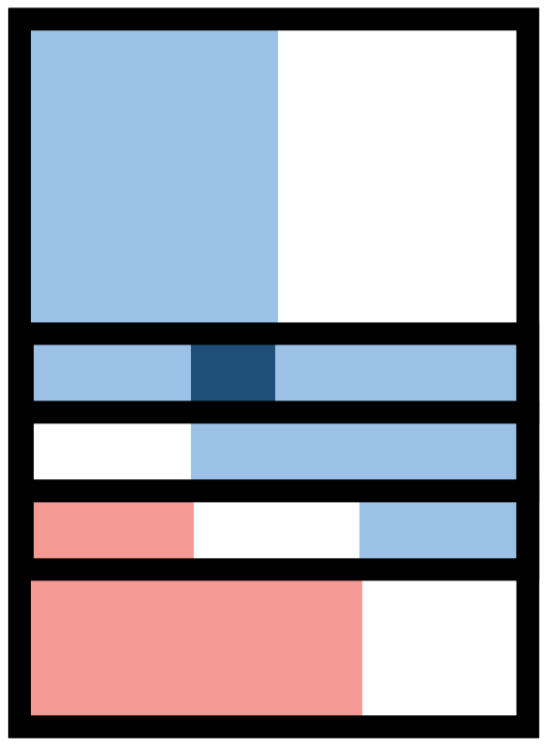
\includegraphics[width=0.2\textwidth]{plots/biclustering_diagrams/rows.png}}
\subfloat[Clustering samples\label{fig:cols}]{
    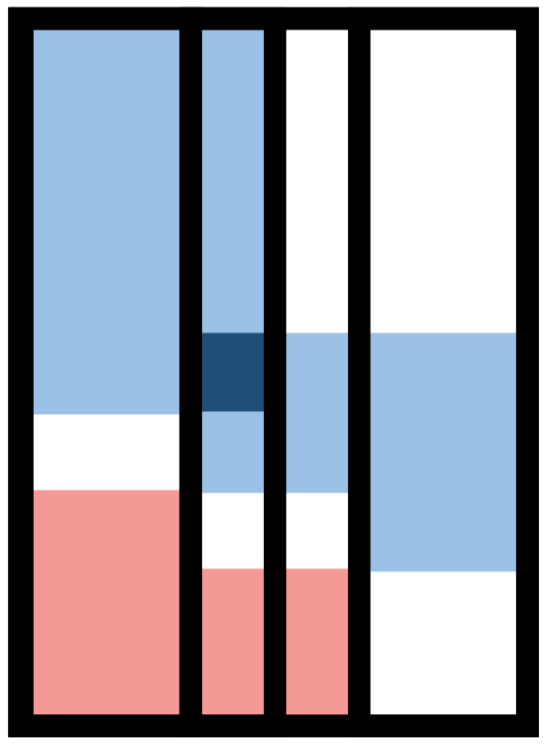
\includegraphics[width=0.2\textwidth]{plots/biclustering_diagrams/cols.png}}
\end{minipage}
\\
\begin{minipage}{1\linewidth}
    \centering
\subfloat[Biclustering\label{fig:biclusters}]{
    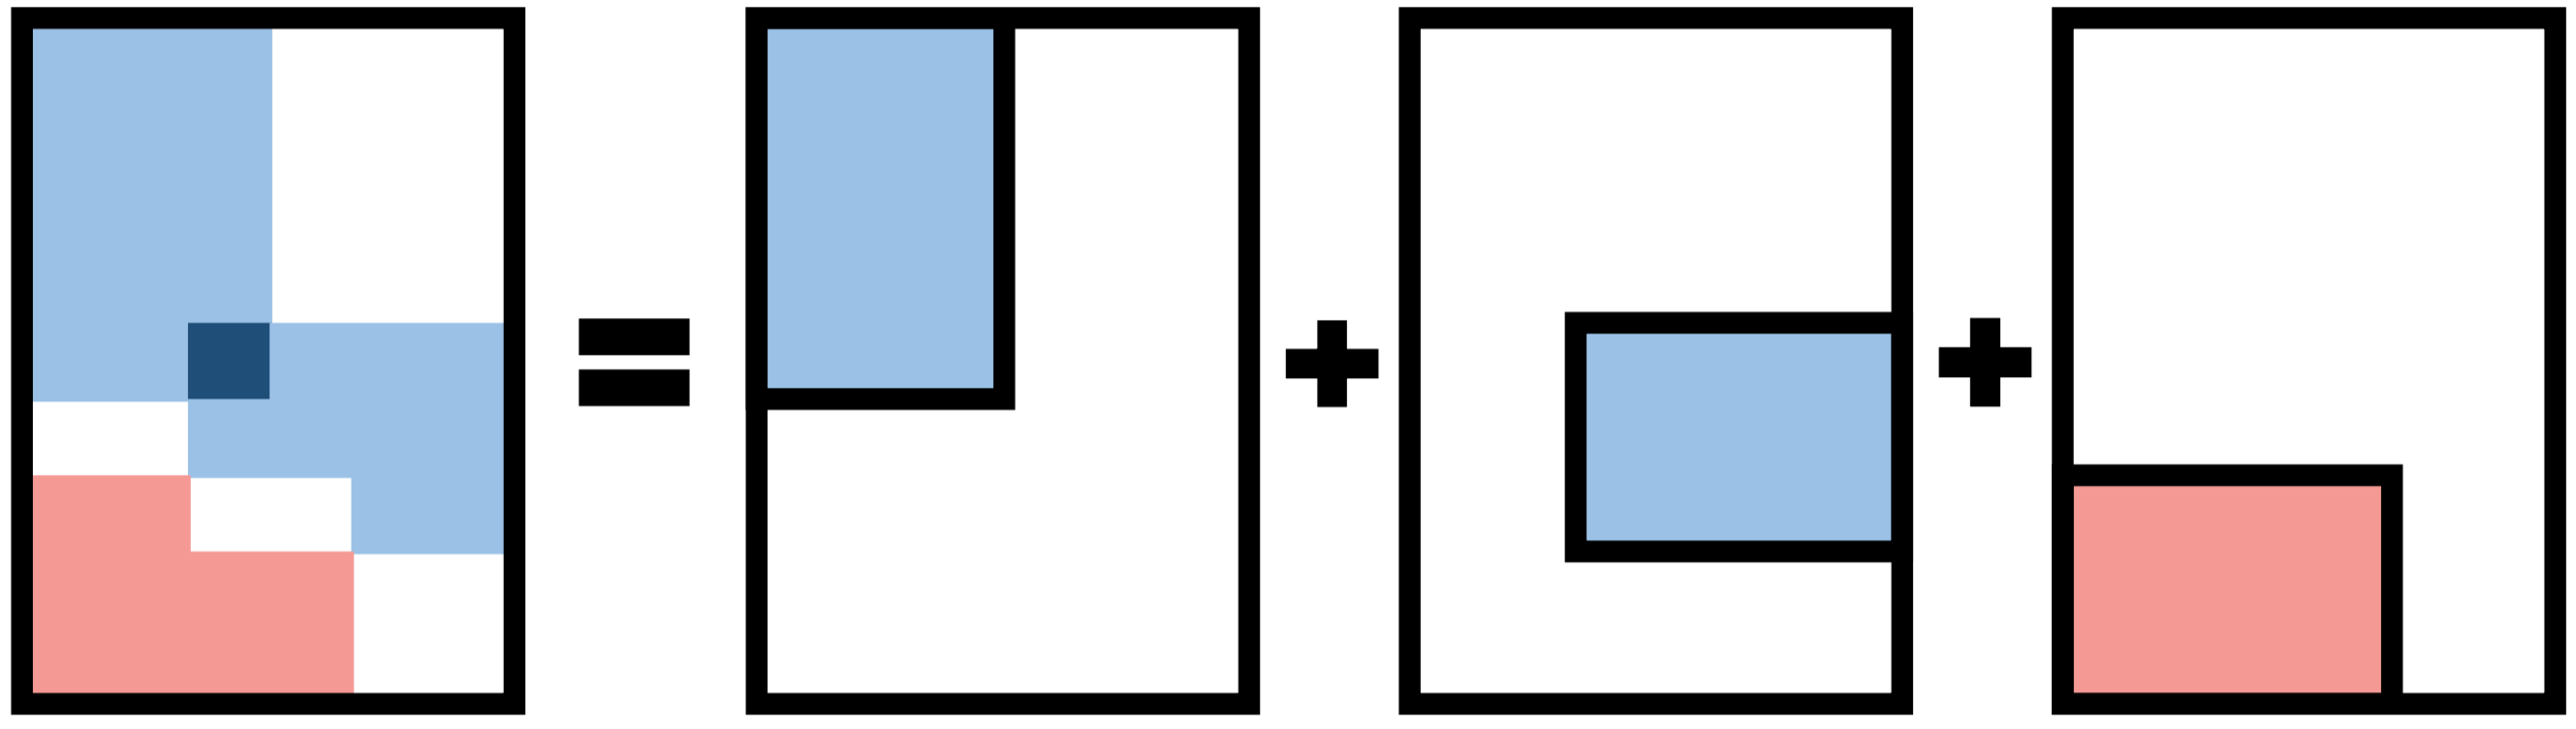
\includegraphics[width=0.85\textwidth]{plots/biclustering_diagrams/biclusters.png}}
\end{minipage}
\caption{The same matrix is used for each type of clustering, with rows as genes and columns as samples. Only biclustering captures the true structure of the dataset.}
\label{fig:caption}
    \end{figure}

\end{block}

%------------------------------------------------

%----------------------------------------------------------------------------------------
%	ALGORITHMS
%----------------------------------------------------------------------------------------

\begin{block}{Algorithm classes}

\begin{table}[t!]
    \caption{Overview of the four classes of biclustering algorithm included.}

    \begin{tabular}{ l | l }
\textbf{Class} & \textbf{Advantages} \\ \hline
    \cellcolor[HTML]{C50F11}\color[HTML]{FFFFFF}\textbf{\textit{Adaptive}} & \multirow{2}{0.6 \textwidth}{Mixture of sparse and dense biclusters, learn K automatically} \\
    SSLB, BicMix & \\ \hline
    \cellcolor[HTML]{3B93DC}\color[HTML]{FFFFFF}\textbf{\textit{NMF}} & \multirow{2}{0.6 \textwidth}{Fast, interpretable} \\
    nsNMF, SNMF & \\ \hline
    \cellcolor[HTML]{50bd4c}\color[HTML]{FFFFFF}\textbf{\textit{Popular}} & \multirow{2}{0.6 \textwidth}{Benchmark - in previous comparison studies} \\
     FABIA, Plaid & \\ \hline
    \cellcolor[HTML]{7f1c8e}\color[HTML]{FFFFFF}\textbf{\textit{Tensor}} & \multirow{2}{0.6 \textwidth}{Share information across cell types} \\
    MultiCluster, SDA & \\ \hline
\end{tabular}
\end{table}

\end{block}


%----------------------------------------------------------------------------------------
%	Study aims
%----------------------------------------------------------------------------------------


\begin{block}{Novel study features}

\begin{itemize}
    \item \bold{Algorithm classes} not previously compared
    \item \bold{Range of complexity} of simulated datasets
    \item \bold{Direct evaluation} of biclustering on \bold{real datasets}
\end{itemize}

\end{block}

%----------------------------------------------------------------------------------------




\end{column} % End of the first column

\begin{column}{\sepwid}\end{column} % Empty spacer column

\begin{column}{\twocolwid} % The second column (double column)

%----------------------------------------------------------------------------------------
%	RESULTS
%----------------------------------------------------------------------------------------

\begin{block}{Results}
\end{block}

% Split this middle column into two
\begin{columns}
\begin{column}{\onecolwid}


\kcnsubheading{Novel thresholding step reveals biclusters}

\begin{itemize}
    \item Raw output had only trivial biclusters containing every gene and every sample
    \item After thresholding, diverse biclusters revealed
    \item Unnecessary for \textit{Adaptive} algorithms
\end{itemize}

\begin{figure}
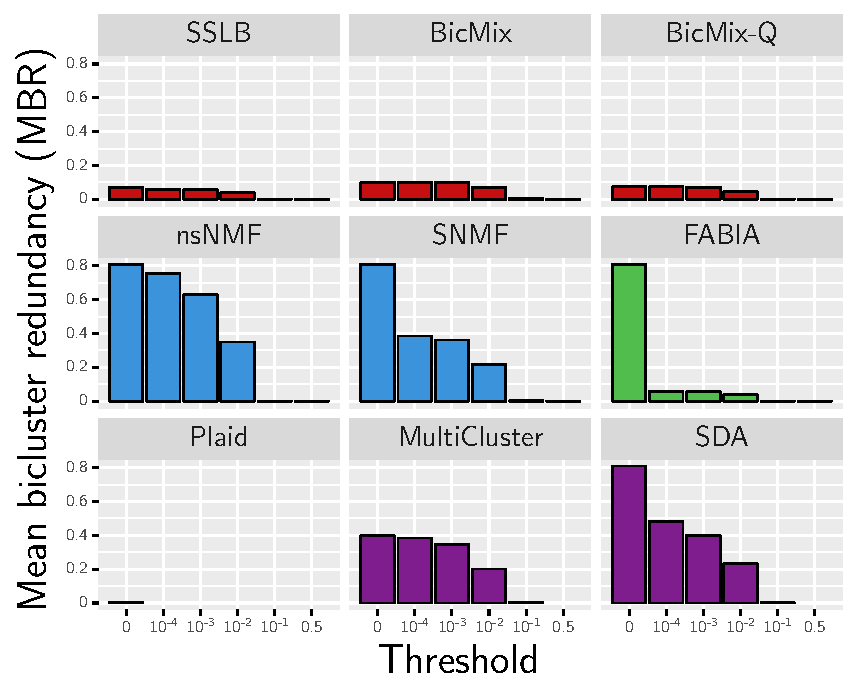
\includegraphics[width=\textwidth]{plots/threshold_adjusted_redundancy_mean.pdf}
\caption{Novel metric MBR (Mean Bicluster Redundancy) measures similarity between biclusters within a run. Lower values preferred. This is shown for different threshold values. Raw output (threshold 0) of FABIA, \textit{NMF} and \textit{Tensor} algorithms contained many copies of same (trivial) biclusters, but after more severe thresholding this improves. We chose threshold $10^{-2}$ for analysis.}
\end{figure}

\kcnsubheading{\textit{Adaptive} algorithms most accurate on simulated datasets}

\begin{itemize}
    \item Using robust metric Clustering Error \cite{horta_similarity_2014}
\end{itemize}

\begin{figure}
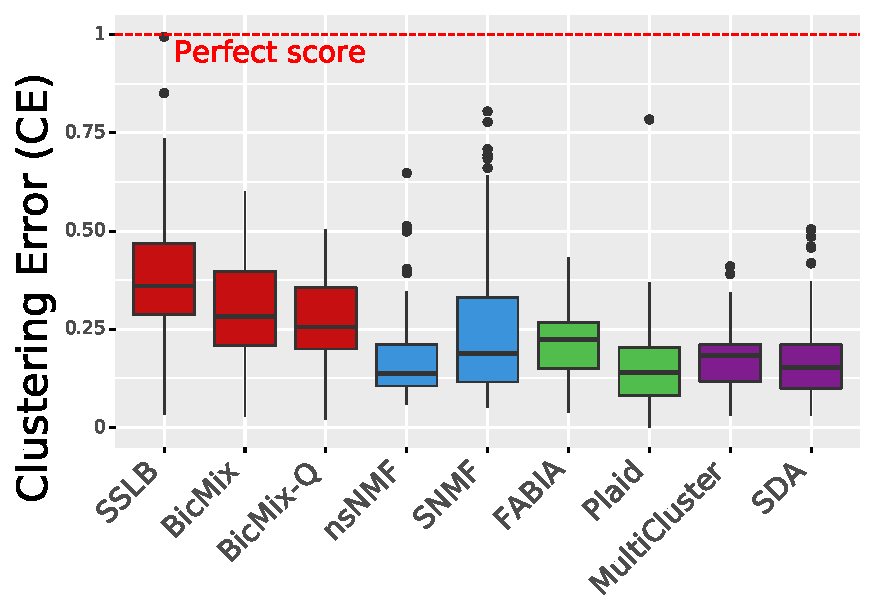
\includegraphics[width=0.9 \textwidth]{plots/summary_clust_err_best_theoretical_K_init.pdf}
\caption{Clustering error (CE) across all simulated datasets. Larger values indicate higher accuracy. $K_\text{init}$ is $K_\text{true}+10$ for \textit{Adaptive} algorithms and $K_\text{true}$ otherwise. Thresholding has been applied. Runs that failed are discarded in the analysis.}
\end{figure}
\end{column} % End of column 2.1

\begin{column}{\onecolwid} % The third column


\kcnsubheading{SSLB, Plaid and \textit{NMF} algorithms best recovery of biclusters in knockout-mouse dataset \cite{koscielny_international_2014}}

\begin{itemize}
    \item Results vary by normalisation method
\end{itemize}

\begin{figure}
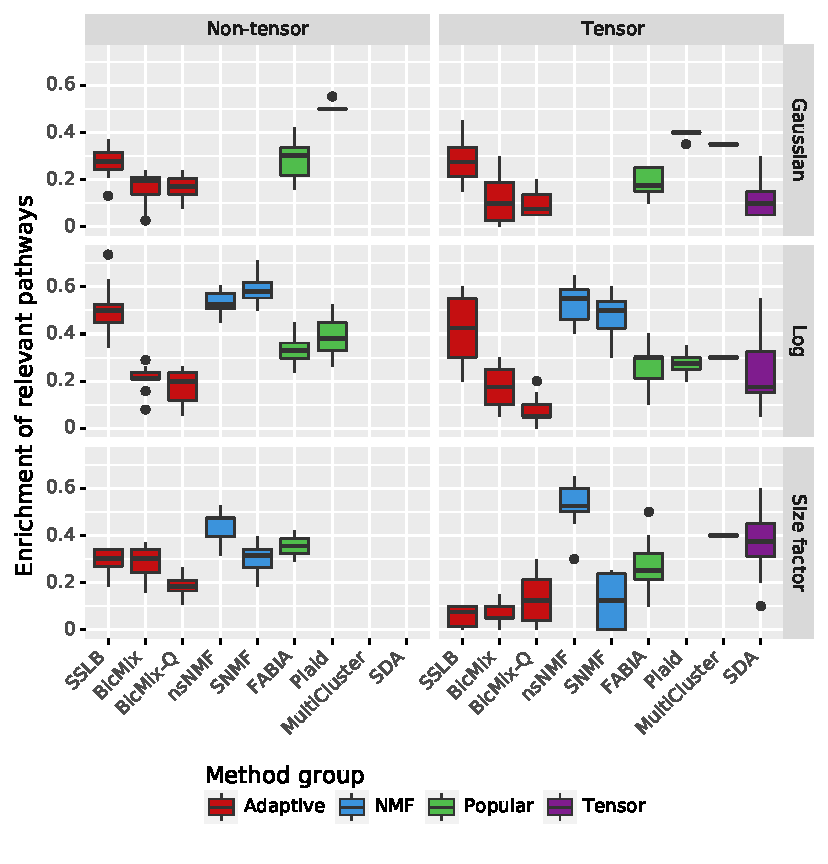
\includegraphics[width=\textwidth]{plots/compare_samegenes_K_50_datasets_ko_traits_nz_alpha_0-05.pdf}
\caption{Bicluster recovery on IMPC knockout-mouse dataset. Measured by mean proportion of knocked-out genes for which the bicluster best matching the samples where the gene was knocked out is enriched for at least one pathway containing the knocked-out gene. The measure is shown for tensor and non-tensor forms of the dataset and three different normalisation methods. \textit{NMF} algorithms can't use Gaussian datasets, \textit{Tensor} algorithms can't use non-tensor datasets.}
\end{figure}


\bigskip
\bigskip
\bigskip
\bigskip


\kcnsubheading{nsNMF fastest, \textit{Adaptive} algorithms slower}

\begin{table}[t!]
\caption{Time in seconds for each algorithm to run on the largest simulated dataset and the main real dataset. Plaid failed to find any biclusters in the largest simulated dataset. Times under 5 minutes are underlined.}

\begin{tabular}{ l | r | r }
    & \multicolumn{2}{c}{\textbf{Time to run (s)}} \\
    \textbf{Algorithm} & \textbf{Simulated} & \textbf{Real} \\ \hline
\cellcolor[HTML]{C50F11}\color[HTML]{FFFFFF}SSLB & 6801 & 3904 \\
\cellcolor[HTML]{C50F11}\color[HTML]{FFFFFF}BicMix & 11250 & 354 \\
\cellcolor[HTML]{C50F11}\color[HTML]{FFFFFF}BicMix-Q & 29587 & 837 \\ \hline
\cellcolor[HTML]{3B93DC}\color[HTML]{FFFFFF}nsNMF & \runnerup{263} & \runnerup{6} \\
\cellcolor[HTML]{3B93DC}\color[HTML]{FFFFFF}SNMF & \runnerup{146} & 29107 \\ \hline
\cellcolor[HTML]{50bd4c}\color[HTML]{FFFFFF}FABIA & 1459 & 749 \\
\cellcolor[HTML]{50bd4c}\color[HTML]{FFFFFF}Plaid & * & \runnerup{90} \\ \hline
\cellcolor[HTML]{7f1c8e}\color[HTML]{FFFFFF}MultiCluster & 696 & \runnerup{40} \\
\cellcolor[HTML]{7f1c8e}\color[HTML]{FFFFFF}SDA & 4746 & 3330 \\

\end{tabular}
\end{table}


\end{column} % End of column 2.2
\end{columns} % End of two columns comprising middle column

%----------------------------------------------------------------------------------------

\end{column} % End of middle (double) column

\begin{column}{\sepwid}\end{column} % Empty spacer column
\begin{column}{\onecolwid} % The fourth column


\kcnsubheading{\textit{NMF} algorithms and Plaid most robust}

\begin{itemize}
    \item Overall fairly low similarity between pairs of runs which differ only by seed
\end{itemize}

\begin{figure}
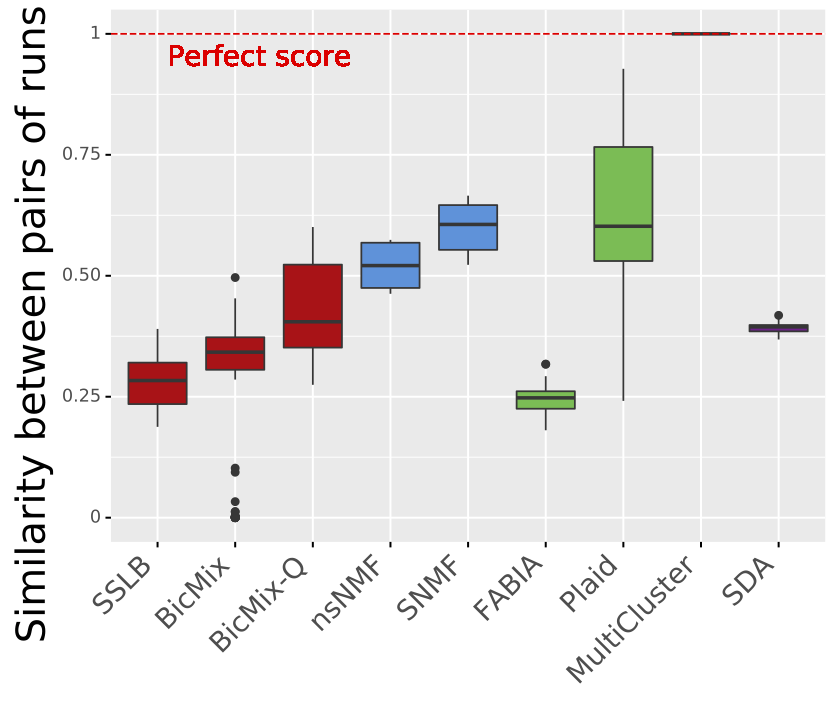
\includegraphics[width=\textwidth]{plots/similarity_methods_K.png}
\caption{Each algorithm was run on the IMPC dataset with 10 different seeds. Plot shows similarity between pairs of such runs for each algorithm, as measured by Clustering Error. It thus gives a measure of robustness of the biclusters recovered by the algorithms.}
\end{figure}

%----------------------------------------------------------------------------------------
%	CONCLUSION
%----------------------------------------------------------------------------------------

\begin{block}{Conclusion}

\begin{itemize}
    \item Novel post-processing thresholding invaluable
    \item \textit{Adaptive} algorithms best for dataset with unknown K and without processing
    \item \textit{NMF} algorithms have potential - fast and robust
\end{itemize}

\end{block}

\begin{alertblock}{Preprint}
For full details, see the preprint on bioRxiv: \\
\small \url{https://doi.org/10.1101/2020.12.15.422852}
\end{alertblock}

%----------------------------------------------------------------------------------------
%	REFERENCES
%----------------------------------------------------------------------------------------

%\begin{block}{References}

%\nocite{*} % Insert publications even if they are not cited in the poster
\printbibliography

%\end{block}

\bigskip
\bigskip

%----------------------------------------------------------------------------------------
%	ACKNOWLEDGEMENTS
%----------------------------------------------------------------------------------------

\begin{center}
\begin{tabular}{ccccc}

\includegraphics[height=22mm]{./Cambridge_University_CMYK.eps} & \hspace{15mm} & 
\includegraphics[height=22mm]{mrc_logo.jpg} & \hspace{15mm} & 
\includegraphics[height=22mm]{wellcome-logo-black.jpg}
\end{tabular}
\end{center}

%----------------------------------------------------------------------------------------

\end{column} % End of the fourth column

\end{columns} % End of all the columns in the poster

\end{frame} % End of the enclosing frame

\end{document}
